\documentclass{article}

% if you need to pass options to natbib, use, e.g.:
     \PassOptionsToPackage{numbers, compress}{natbib}
% before loading neurips_2021

% ready for submission
%\usepackage{neurips_2021}

% to compile a preprint version, e.g., for submission to arXiv, add add the
% [preprint] option:
     \usepackage[preprint]{neurips_2021}

% to compile a camera-ready version, add the [final] option, e.g.:
%     \usepackage[final]{neurips_2021}

% to avoid loading the natbib package, add option nonatbib:
%    \usepackage[nonatbib]{neurips_2021}

\usepackage[utf8]{inputenc} % allow utf-8 input
\usepackage[T1]{fontenc}    % use 8-bit T1 fonts
\usepackage{hyperref}       % hyperlinks
\usepackage{url}            % simple URL typesetting
\usepackage{booktabs}       % professional-quality tables
\usepackage{amsfonts}       % blackboard math symbols
\usepackage{nicefrac}       % compact symbols for 1/2, etc.
\usepackage{microtype}      % microtypography
\usepackage{xcolor}         % colors
\usepackage[labelfont=bf]{caption}
\usepackage{graphicx}    % inserting images
\bibliographystyle{unsrtnat}

\title{Convergence of Optimizers Without Bounded Gradient Assumption}

% The \author macro works with any number of authors. There are two commands
% used to separate the names and addresses of multiple authors: \And and \AND.
%
% Using \And between authors leaves it to LaTeX to determine where to break the
% lines. Using \AND forces a line break at that point. So, if LaTeX puts 3 of 4
% authors names on the first line, and the last on the second line, try using
% \AND instead of \And before the third author name.

\author{%
  Roger Wang \ \ \ \  Eric Xia \\
  University of Washington\\
  \texttt{\{rogerwyf, ericxia\}@uw.edu} 
}
\usepackage{enumitem}
\usepackage{mathtools}
\usepackage{hyperref}
\usepackage{xcolor}
\hypersetup{
	colorlinks,
	linkcolor={black!50!black},
	citecolor={blue!50!black},
	urlcolor={blue!80!black}
}

\newtheorem{theorem}{Theorem}[section]
\newtheorem{corollary}{Corollary}[section]
\newtheorem{lemma}[theorem]{Lemma}
\newtheorem{definition}{Definition}[section]

\begin{document}

\maketitle

%\begin{abstract}
%\end{abstract}

\section{Introduction}

The primary goal of most deep learning models is to minimize the underlying loss function.
Optimizers are crucial for the task of updating model weights such that the model will actually converge to a minimum in a computationally efficient manner instead of overshooting or moving away from the minimum. While existing optimizers are intuitively straightforward in convex learning, in non-convex settings they (notably for Adam-type adaptive gradient methods)
often require the assumption on the boundedness of gradients for achieving convergence.

While convenient, the imposition of assumptions on the boundedness of gradients can be difficult to verify in practical settings, hence in recent years there has been a trend in research efforts towards analyzing existing optimization methods and proposing novel methods without such assumptions. 

In this report, we will review four recent research papers on the convergence of stochastic optimization algorithms including SGD (\hyperref[section3]{Section 3}), SGD with Momentum (\hyperref[section4]{Section 4}), Root Mean Squared Propagation (RMSProp) (\hyperref[section6]{Section 5}) and Adaptive Moment Estimation (Adam) (\hyperref[section7]{Section 6}), analyzing their approaches, methodologies, and findings as well as discussing their broader implications for the convergence problem and the general field of optimizers.
\section{General Assumptions}
In a stochastic setting, the optimization problem for a neural network training process can be written as a finite-sum problem:
\[
\min_{x \in \mathbb{R}^d} f(x) = \frac{1}{n}\sum_{j = 0}^{n - 1} f(x, s_j)
\]
where $f(x, s_j)$ represents the loss function contributed by the randomly shuffled sample batch $s_j$.\\
\newline
Let $g_t\coloneqq\nabla f(x_t)$ and $\tilde{g}_t \coloneqq  \nabla f(x_t, s_t)$ be the full gradient and the stochastic gradient with respect to the sampled batch $s_t$ of the objective function $f$ at time or iteration $t$, respectively. Below we list the common assumptions in standard stochastic optimization that are either explicitly stated or implied in the papers covered in this report:
\begin{enumerate}[leftmargin=*]
	\item \textit{\textbf{Lower boundedness}: $f$ is lower-bounded by some function $f^*$.}
	\item \textit{\textbf{Smoothness}: $f$ is $L$-smooth or $\nabla f$ is $L$-Lipschitz continuous for some constant $L$.}
	\item \textit{\textbf{Unbiased gradients}: $\forall t, \mathbb{E}_{s_t}[\tilde{g}_t] = g_t$}.
	\item \textit{\textbf{Independence}: the random samples $s_j$'s are independent.}
	\item \textit{\textbf{Bounded variance}: $Var_{s_t}(\tilde{g}_t) = \mathbb{E}_{s_t}[\tilde{g}_t - g_t] \leq \sigma^2$ for some $\sigma > 0$.}
\end{enumerate}
\textbf{Throughout this report, we will refer to the above as \textit{General Assumptions} and use the above notations}.
It is worth mentioning that none of these assumptions is related to the boundedness to gradient $g_t$ or $\tilde{g}_t$, which is often the key assumption utilized by previous theoretical work.
\section{Stochastic Gradient Descent for Structured Nonconvex Functions}
\label{section3}
\subsection{Previous Research \& Motivation}

Prior to~\cite{https://doi.org/10.48550/arxiv.2006.10311}, standard convergence theory for SGD in smooth non-convex settings gave a slow sublinear convergence to a stationary point. There has recently been a great interest
in exploiting additional structure of classes of nonconvex function, such as error bound properties~\cite{Fabian2010ErrorBN},
quasi (strong) convexity~\cite{https://doi.org/10.48550/arxiv.1906.11985, JMLR:v19:16-465, https://doi.org/10.48550/arxiv.1710.00797}, and quadratic growth condition~\cite{doi:10.1137/S1052623499359178}.

In~\cite{https://doi.org/10.48550/arxiv.2006.10311}, Gower et al. provide a new general analysis of SGD focusing on the two weakest of these properties, quasar (strongly) convex (QC) functions and functions satisfying the
Polyak-Łojasiewicz (PL) conditions~\cite{POLYAK1963864}, using the expected residual (ER) condition~\cite{Gower2021StochasticQM}.

\subsection{Additional Assumptions}
On top of \textit{General Assumptions}, the paper assumes that the \textit{gradient noise} $\sigma^2$ is finite and that the Expected Residual condition holds, where $g\in\text{ER}(\rho)$ if
\begin{equation}
	\label{eq31}
	\mathbb{E}\left[||g(x) - g(x^*) - (\nabla f(x) - \nabla f(x^*))||^2\right] \leq 2\rho (f(x) - f(x^*)), \ \ \forall x\in\mathbb{R}^d.
\end{equation}

\subsection{Main Results \& Methodology}
The main results of the paper are convergence bounds using the ER condition for SGD on QC functions and minibatch SGD on PL functions.
\begin{theorem}[QC Functions with Constant and Decreasing Step-sizes]
	\label{them31}
	Assume \textit{General Assumptions}, $f(x)$ is $\zeta$-QC with respect to $x^*$, and $g\in\text{ER}(\rho)$. Let $0 < \gamma_k < \frac{\zeta}{2\rho + L}$ for all $k\in\mathbb{N}$ and let $r_0\coloneqq ||x^0 - x^*||^2$.
	Then iterates of SGD satisfy
	\[
		\substack{\min \\ t=0,\dots, k-1}\mathbb{E}\left[f(x^t) - f(x^*)\right] \leq \frac{1}{\sum_{i=0}^{k-1}}\gamma_i (\zeta - \gamma_i (2\rho + L)) \left[\frac{r^0}{2} + \sigma^2 \sum^{k-1}_{t=0}\gamma_t^2\right].
	\]

	Furthermore, for $\gamma < \frac{\zeta}{2\rho + L}$, we have that

	\textbf{1}. If $\forall k\in\mathbb{N}$, $\gamma_k = \gamma \equiv \frac{1}{2}\frac{\zeta}{(2\rho + L)}$ then $\forall k\in\mathbb{N},\ \substack{\min \\ t=0,\dots, k-1}\mathbb{E}[f(x^t) - f(x^*)]\leq 2r_0 \frac{2\rho + L}{\zeta^2 k} + \frac{\sigma^2}{2\rho + L}$. \\
	\textbf{2}. Suppose SGD is run for $T$ iterations. If $\gamma_k = \frac{\gamma}{\sqrt{T}}$ for all $k$ from 0 to $T-1$, then\\
	\makebox[\textwidth]{$\substack{\min \\ t=0,\dots, T-1} \mathbb{E}[f(x^t) - f(x^*)] \leq \frac{r_0 + 2\gamma^2 \sigma^2}{\gamma\sqrt{T}}$}
	\textbf{3}. If $\forall k\in\mathbb{N},\ \gamma_k = \frac{\gamma}{\sqrt{k+1}}$ then $\forall k \in\mathbb{N}$, \\
	\makebox[\textwidth]{$\substack{\min \\ t=0,\dots, k-1} \mathbb{E}[f(x^t) - f(x^*)] \leq \frac{1}{4\gamma} \frac{r_0 + 2\gamma^2 \sigma^2 (\log{(k)} + 1)}{\zeta (\sqrt{k} - 1) - \gamma(\rho + L/2)(\log{(k)} + 1)}$,}
	which converges at a rate $\mathcal{O}\left(\frac{\log(k)}{\sqrt{k}}\right)$.
\end{theorem}

\begin{theorem}[PL Functions with Constant Step-sizes]
	\label{them32}
	Assume \textit{General Assumptions}, $f\in\text{PL}(\mu)$, and $g\in\text{ER}(\rho)$. Let $\gamma_k = \gamma\leq \frac{1}{1+2\rho/\mu}\frac{1}{L}$, for all $k$, then SGD converges as follows:
	\begin{equation}
		\label{eq32}
		\mathbb{E}[f(x^k) - f^*] \leq (1-\gamma\mu)^k[f(x^0) - f^*] + \frac{L\gamma\sigma^2}{\mu}.
	\end{equation}
	Thus, given $\epsilon > 0$ and using step size $\gamma = \frac{1}{L}\min\{\frac{\mu\epsilon}{2\sigma^2}, \frac{1}{1+2\rho/\mu}\}$ we have that
	\begin{equation}
		\label{eq33}
		k\geq \frac{L}{\mu}\max\Big\{\frac{2\sigma^2}{\mu\epsilon}, 1+\frac{2\rho}{\mu}\Big\}\log\left(\frac{2(f(x^0) - f^*)}{\epsilon}\right) \implies \mathbb{E}[f(x^k) - f^*]\leq \epsilon.
	\end{equation}
	When the function interpolates the data, SGD converges to the solution at a linear rate.
\end{theorem}

We will now elaborate on the methodology used to achieve the results. Taking $z=x-\frac{1}{L}(\nabla f(x) - \nabla f(x^*))$ for any $x,z\in\mathbb{R}^d$ that defines $L$-smoothness of $f$, the definition for $L$-smooth may be rearranged st.
\begin{equation}
	\label{eq34}
	||\nabla f(x)||^2 \leq 2L(f(x) - f(x^*)).
\end{equation}

Using this and the definitions of Strong Growth Condition + L-smooth, Weak Growth Condition, Expected Smoothness, and ER in that successive order, it follows from simple rearrangements and taking expectations that this order also gives the descending strength of the concerned assumptions.

Using \hyperref[eq31]{(1)} and \hyperref[eq34]{(4)} together gives
\begin{equation}
	\mathbb{E}_D\left[||g(x)||^2\right]\leq 2(2\rho + L)(f(x) - f(x^*)) + 2\sigma^2,
\end{equation}
where $g\in\text{ER}(\rho)$ and $x\in\mathbb{R}^d$. With an unbiased estimate of the gradient $g(x)$ we can then use SGD to solve the unconstrained finite-sum optimization problem by sampling $g(x^k)$ i.i.d. and iterating
\[x^{k+1} = x^k - \gamma^k g(x^k).
\]
We have
\[||x^{k+1} - x^*||^2 = ||x^k - x^*||^2 - 2\gamma_k \langle g(x^k), x^k - x^*\rangle + \gamma_k^2 ||g(x^k)||^2.
\]
By rearranging and taking expectation, then summing over $k=0, \dots, t-1$ and using telescopic cancellation, we have that iterates of SGD satisfy the equation in \hyperref[them31]{Theorem 3.1} and the remaining conclusions in \hyperref[them31]{Theorem 3.1} follow by substitutions and integral bounds.
For \hyperref[them32]{Theorem 3.2}, smoothness of $f$ is combined with SGD update rule, where expectation conditioned on $x^k$ is taken and the resultant geometric series summed to get \hyperref[eq32]{(2)}. Dividing the RHS of \hyperref[eq32]{(2)} into two parts and bounding each separately by $\frac{\epsilon}{2}$, we restrict
the step size as in \hyperref[them32]{Theorem 3.2} and insert $\gamma$ into a rearrangement of these bounds to get \hyperref[eq33]{(3)}.

\subsection{Discussion}

The ER condition relies solely on $L$-smoothness of $f$ and interpolation of data points and is shown above to be strictly weaker than previous assumptions, including the bounded gradient. Not only does ER hold for a larger class of assumptions than standard convergence theory in nonconvex setting which relies on bounded gradient assumption~\cite{https://doi.org/10.48550/arxiv.1106.5730, JMLR:v15:hazan14a, Rakhlin2012MakingGD} or a growth condition~\cite{Bertsekas1995NeurodynamicPA, https://doi.org/10.48550/arxiv.1606.04838, Schmidt2017MinimizingFS},
resulting convergence rates either match or exceed state-of-the-art for both QC and PL functions.
Recent evidence suggests a QC structure for loss functions in NNs~\cite{Zhou2019SGDCT} and this work recovers a $O(1\sqrt{k})$ convergence rate for QC functions with only the ER assumption.

For PL functions, SGD was previously shown to converge at a rate of $O(1/\sqrt{k})$ assuming bounded gradients~\cite{Karimi2016LinearCO}. Assuming in addition the interpolation and SGC, a linear rate was achieved in Vaswani et al. 2019, but with a suboptimal dependence on the condition number
of the function. This work achieves linear convergence to a neighborhood for PL functions.

Recently, Khaled and Richtarik (2020)~\cite{https://doi.org/10.48550/arxiv.2002.03329} present convergence analysis of SGD in nonconvex setting, relying on the ABC assumption (\textit{\hyperref[eqa1]{equation A.1} in Appendix}),
of which all previously discussed assumptions SGC, WGC, ES, and ER are special cases by taking different values for $A,B,C$. Whereas
\hyperref[them32]{Theorem 3.2} above is less general and therefore stronger than Theorem 3 in Khaled and Richtarik's work, unlike~\cite{https://doi.org/10.48550/arxiv.2002.03329}, \hyperref[them32]{Theorem 3.2} does not depend on total number of steps and this allows practitioners to simply
observe SGD progress and stop when a desired tolerance is achieved.

\section{Stochastic Gradient Descent with Momentum}
\label{section4}
\subsection{Previous Research \& Motivation}
\setcounter{equation}{0}
Prior to~\cite{NEURIPS2020_d3f5d4de} by Liu et al., there had been some interests in investigating the convergence of SGDM.~\cite{https://doi.org/10.48550/arxiv.1905.03817} provides a global convergence of SGDM but it assumes uniformly boundedness of gradients of the objection funcion.~\cite{https://doi.org/10.48550/arxiv.1808.10396} presents a convergence bound of SGDM for general nonconvex functions but does not explain the competitiveness of SGDM compared to SGD.
Moreover, the convergence rate of Multistage SGDM had not been established except for the classic SGD case.

In this work, Liu et al. provide a novel convergence analysis for SGDM and
Multistage\footnote{Multistage refers to applying a constant stepsize which is then dropped by a constant factor to encourage fine-tuning of training, and the momentum weight is either kept unchanged or gradually increased.}
SGDM without bounded gradient assumptions. This work also demonstrates that SGDM has the same convergence bound as SGD for both strongly convex and nonconvex functions without uniformly bounded gradient assumption,
and is the first convergence guarantee for SGDM in a multistage setting.

\subsection{Main Results \& Methodology}
The main results of this paper are the convergence bounds of SGDM and Multistage SGDM. In SGDM, let $\alpha$ and $\beta$ be learning rate and momentum weight, we have the following result:
\begin{theorem}[Non-convex SGDM]
	\label{theom41} Assume $f:\mathbb{R}^d \rightarrow \mathbb{R}$ satisfies General Assumptions, let $\alpha \leq \min\{\frac{1 - \beta}{L(4 - \beta + \beta^2)}, \frac{1 - \beta}{2\sqrt{2}L\sqrt{\beta + \beta^2}}\}$, then
	\[\frac{1}{k}\sum_{i = 1}^{k}\mathbb{E}[\|g_t\|^2] \leq \frac{2 (f(x_1) - f^*}{k\alpha} + (\frac{\beta + 3\beta^2}{2 (1 + \beta)} + 1)L\alpha\sigma^2 = \mathcal{O}(\frac{f(x_1) - f^*}{k\alpha} + L\alpha\sigma^2)
	\]
\end{theorem}
\begin{theorem}[Strongly Convex SGDM]
	\label{theom42} Assume $f:\mathbb{R}^d \rightarrow \mathbb{R}$ satisfies General Assumptions and is $\mu$-strongly convex, let $\alpha \leq \min\{\frac{1 - \beta}{5L}, \frac{1 - \beta}{L(3 - \beta + 2\beta^2 + \frac{48\sqrt{\beta}}{25}\frac{2L + 18\mu}{L})}\}$, then for all $t \geq t_0:= \lfloor\frac{\log 0.5}{\log \beta}\rfloor$, 
	\[
		\mathbb{E}[f(x_t) - f^*] = \mathcal{O}\bigl(\max\{1 - \alpha\mu, \beta\} + \frac{L}{\mu}\alpha\sigma^2\bigr)
	\]
\end{theorem}
In a multistage setting, let $\alpha_i$, $\beta_i$ and $T_i$ are learning rate (step size), momentum weight and stage length of $i$th stage, respectively, we have the following result:
\begin{theorem}[Non-convex Multistage SGDM]
	\label{theom43} Assume $f:\mathbb{R}^d \rightarrow \mathbb{R}$ satisfies General Assumptions, restrict the parameters in each stage of Multistage SGDM so that 
\begin{equation}
\label{eq41}
\frac{\alpha_i\beta_i}{1 - \beta_i} \equiv A_1, \alpha_iT_i \equiv A_2 \ \ \text{for}  \ \ i = 1,...,n \ \ \ \text{and} \ \ \
0 \leq \beta_1 \leq \beta_2 \leq ... \leq \beta_n \leq 1
\end{equation}
and $A_1, A_2$ are properly chosen constants. Let $A_1 = \frac{1}{24\sqrt{2}L}$ and $A_2$ be large enough so that $\beta_i^{2T_i} \leq \frac{1}{2}$ for $i = 1,...,n$. In addition, let
\[
\frac{1 - \beta_1}{\beta_1} \leq 12 \frac{1 - \beta_n}{\sqrt{\beta_n + \beta_n^2}}
\] then we have
\[
\begin{split}
\frac{1}{n}\sum_{l = 1}^{n}\frac{1}{T_l}\sum_{i = T_1 + ... + T_{l - 1} + 1}^{T_1 + .. + T_l}\mathbb{E}[\|g_t\|^2] &\leq \frac{2(f(x_1) - f^*)}{nA_2} + \frac{1}{n}\sum_{i = 1}^n\Bigl(24\beta^2_l\frac{\beta_1}{\sqrt{\beta_n + \beta_n^2}L + 3L}\Bigr)\alpha_l\sigma^2\\
&= \mathcal{O}\Bigl(\frac{2(f(x_1) - f^*)}{nA_2} + \frac{1}{n}\sum_{i = 1}^nL\alpha_l\sigma^2\Bigr)
\end{split}
\]
\end{theorem}
Next, we will summarize the key approaches used to derive the above results. Recall that the core of SGDM algorithm is the following updating rule:
\[
v_t = \beta v_{t - 1} + (1 - \beta)\tilde{g}_t \ \ \ \
x_{t + 1} = x_t - \alpha v_t
\]
Therefore, assume $v_0 = 0$, then $v_t$ can be expressed as 
\begin{equation}
\label{eq42}
v_t = (1 - \beta)\sum_{i = 1}^{t}\beta^{k - i}\tilde{g}_i
\end{equation}
One key observation on the role of $\beta$ in equation (\hyperref[eq42]{2}) from the paper is that $v_t$ enjoys a reduced variance of $(1 - \beta)\sigma^2$ while having a controllable deviation from the full gradient $g_t$ in expectation since $v_t$ is a moving average of the past stochastic gradients with lower weights on the older ones, thus it makes sense to look at the deterministic version of $v_t$ (replacing $\tilde{g}_i$ with $g_i$) and its deviation from the ideal descent direction $g_t$, which could be unbounded without further assumptions.

While previous work assumed the boundedness of $g_t$ to circumvent above difficulty, this work constructed a novel Lyapunov function to handle this deviation:
\[
L_t = (f(z_t) - f^*) + \sum_{i = 1}^{k - 1}c_i\|x^{k + 1 - i} - x^{k - i}\|^2 \ \
\text{with} \ \  z_t = \begin{cases}
	x_t & t = 1 \\
	\frac{1}{1 - \beta}x_t - \frac{\beta}{1 - \beta}x_{t - 1} & t \geq 2
\end{cases}
\]

The authors then argued that by carefully defining $\{c_i\}_i^\infty$ such that it is a positive sequence in a diminishing fashion, $L_t$ is indeed a Lyapunov function, thus one can show that $\mathbb{E}[L_{t + 1} - L_t] \leq -R_1E[\|g_t\|^2] + R_2$ for some positive constants $R_1 \geq \frac{\alpha}{2}$ and $R_2 = \mathcal{O}(L\alpha\sigma^2)$. By telescoping this inequality, the convergence of SGDM in \hyperref[theom41]{Theorem 4.1} is then obtained, and similar techniques were utilized to derive the results in \hyperref[theom42]{Theorem 4.2} under a strongly convex setting and in \hyperref[theom43]{Theorem 4.3} for Multistage SGDM.
\subsection{Discussion}
\hyperref[theom41]{Theorem 4.1} and \hyperref[theom42]{Theorem 4.2} show that under both nonconvex and strongly convex settings, with a proper learning rate $\alpha$, SGDM can achieve the same convergence bound as the classical convergence bound of SGD (as shown in previous work, e.g., Theorem 4.5 and 4.8 in~\cite{https://doi.org/10.48550/arxiv.1606.04838}). This result only depends on General Assumptions, and the radius of the stationary distribution is smaller than the previous $\mathcal{O}(\frac{\alpha\sigma^2}{1 - \beta})$ result from~\cite{https://doi.org/10.48550/arxiv.1905.03817} that relies on the additional assumption of uniformly bounded gradients. It is also worth mentioning that the use of Lyapunov function is a novel approach for convergence analysis of optimization algorithms and provides some new insights throughout this paper. 

For Multistage SGDM, \hyperref[theom42]{Theorem 4.3} is the first theoretical result that guarantees its convergence. Moreover, it was demonstrated from the convergence bound that large learning rates are allowed in the first a few stages to accelerate the initial convergence, and smaller learning rates can refine the radius of the stationary distribution in the later stages, which is an advantage of stagewise training compared to plain SGDM.

However, the convergence analysis in this paper does have some weaknesses and limitations: First of all, although it is theoretically shown that SGDM is "at least as fast as" SGD, this paper did not explore the advantages of SGDM compared to SGD in detail. In addition, \hyperref[theom42]{Theorem 4.2} assumes a lower-bound of timestamp/iteration for the result to be valid, and this lower-bound could be a problem for some choices of $\beta$ (e.g, when $\beta = 0.995$, $t_0 = 138$). Finally, equation (\hyperref[eq41]{1}) from \hyperref[theom43]{Theorem 4.3} puts a strong restriction on the choice of learning rates and momentum weights at all stages, which makes this stage-wise training setup impractical.
\section{RMSProp}
\label{section6}
\setcounter{equation}{0}
\subsection{Previous Research \& Motivation}
Prior to~\cite{shi2021rmsprop} by Shi et al., there had been one line of research on the convergence of variants of Adam (which includes RMSProp) with additional assumptions.~\cite{https://doi.org/10.48550/arxiv.2003.02395} provides a clean convergence result but assumed a large $\epsilon$ compared to  weighted moving average of the squared gradient, which is in contrary to the spirit of RMSProp.~\cite{https://doi.org/10.48550/arxiv.1807.06766} analyzes deterministic and stochastic RMSprop, but their results were based on an rather unrealistic assumption that all stochastic gradients have the same sign. Furthermore, all the above mentioned works assume the gradients to be bounded.

During the review on one famous counter-example to the convergence of Adam from~\cite{https://doi.org/10.48550/arxiv.1904.09237}, Shi et al. ran simulations and found that there is always a threshold of the moving average parameter above which
RMSProp converges (See \hyperref[fig1]{Figure 1} in Appendix). This observation motivated them to further investigate the relationship between this parameter and the performance of the algorithm. They discovered that the convergence of RMSProp algorithm is
contingent to the choice of the moving average parameter. Moreover, they proved that RMSProp converges to stationary points for certain types of problems and to bounded region for the others, which was the first result of convergence
of this algorithm with no assumption about the boundedness of the gradient norm.

\subsection{Additional Assumptions}
In addition to \textit{General Assumptions}, this paper assumes that for stochastic RMSProp, the objective satisfies
\begin{equation}
\label{eq51}
\sum_{j = 0}^{n - 1} \|\nabla f_j(x)\|_2^2 \leq D_1 \|\nabla f(x)\|_2^2 + D_0
\end{equation}
for some non-negative constant $D_0$ and $D_1$. This can be viewed as an augment to the bounded variance assumption.
\subsection{Main Results \& Methodology}
The main results of this paper are the convergence of RMSProp under both deterministic and stochastic setting. Let $\alpha_t$  be the learning rate at time/iteration $t$ and $\beta$ be the moving average parameter of the squared gradients norm, we have the following results: 
\begin{theorem}[Deterministic RMSProp]
	\label{theom51}
Assume $f:\mathbb{R}^d \rightarrow \mathbb{R}$ satisfies General Assumptions, then for deterministic RMSProp (i.e, full-batch with $n = 1$, $\epsilon = 0$) with a diminishing learning rate $\alpha_t = \frac{\alpha_1}{\sqrt{t}}$ and any $\beta \in (0, 1)$, we have
\[
\min_{t \in (1, T]} \|g_t\|_1 \leq \mathcal{O}\Big(\frac{\log T}{\sqrt{T}}\Big)
\]
\end{theorem}
where $T > 0$ is the total number of iterations.
\begin{theorem}[Stochastic RMSProp - Bounded Region]
	\label{theom52}
	Assume $f:\mathbb{R}^d \rightarrow \mathbb{R}$ satisfies General Assumptions and (\hyperref[eq51]{1}). In addition, assume $\beta$ satisfies
	\[
	\sqrt{\frac{10dn}{\beta^n}}dnD_1\Big((1 - \beta)\frac{\frac{4n^2}{\beta^n} - 1}{2} + (\frac{1}{\sqrt{\beta^n}}- 1)\Big)\leq \frac{\sqrt{2} - 1}{2\sqrt{2}}
	\]
	Then, for stochastic RMSProp with a diminishing learning rate $\alpha_t = \frac{\alpha_1}{\sqrt{t}}$, we have
	\[
	\min_{t \in (1, T]} \min\{\|\tilde{g}_t\|_1, \|\tilde{g}_t\|_2^2\sqrt{\frac{D_1d}{D_0}}\} \leq \mathcal{O}\Big(\frac{\log T}{\sqrt{T}}\Big) + \mathcal{O}\Big(C\sqrt{D_0}\Big), \ \ \ \forall \ T\geq 4
	\]
	where $C$ is a $\beta$-dependent constant that satisfies $\lim\limits_{\beta \rightarrow 1} C = 0$
\end{theorem}
\begin{corollary}[Stochastic RMSProp - Stationary Point]
	\label{coro51}
	See \hyperref[coro51appendix]{Corollary A.1} in Appendix
\end{corollary}
Next, we explain the methodology used to derive the above results. Recall that the core of the RMSProp algorithm is the following updating rule:
\[
v_t = \beta v_{t - 1} + (1 - \beta)(g_t \circ g_t)\ \  \ \ \ x_t = x_{t - 1} - \alpha(v_t + \epsilon I)^{-1/2}g_t
\] 
For the full-batch version of RMSProp, \hyperref[theom51]{Theorem 5.1} is an extension of results from the original Adam paper~\cite{Gower2021StochasticQM} for which the authors utilized the Lipschitz continuity of the gradients to remove the bounded assumption.\\
\newline
The derivation to the results for stochastic RMSProp is more complicated: Based on the observation from the simulation, the authors divided stochastic optimization problems into two classes: \textit{realizable} problems when $D_0 = 0$ from equation (\hyperref[eq51]{1}) and  \textit{non-realizable} problems when $D_0 \neq 0$. They further conjectured that these two classes of problems correspond to different convergence behavior of RMSProp contingent to the choice of beta, which is summarized in Table \hyperref[tb1]{1}:
\begin{table}[h]
\label{tb1}
\centering
\begin{tabular}{c|c | c}
	\hline
	Class & $\beta$ close to 1 & $\beta$ close to 0\\
	\hline
	Non-realizable & Convergence to bounded region (\hyperref[theom51]{Theorem 5.2}) & Divergence\\
	Realizable & Convergence to stationary points (\hyperref[coro51]{Corollary 5.1}) & Divergence\\
	\hline
\end{tabular}
\vspace{1mm}
\caption{Conjecture on convergence outcomes of RMSProp on classes of optimization problems.}
\vspace{-8mm}
\end{table}
\newline
The rationale to prove this conjecture is to track the magnitude of squared gradient terms and calculate the diminishing speed of $\|g\|_1$. Since $f$ is $L$-Lipschitz, by descent lemma, one can show the following inequality
\begin{equation}
\label{eq52}
f(x_{t + 1}) - f(x_{t}) \leq \langle g_t, x_{t + 1} - x_{t}\rangle + \frac{L}{2}\|x_{t + 1} - x_{t}\|^2
\end{equation}
By examining the distribution of gradient norms among different sampled batches, one can find upper and lower bounds of the inner product between the gradient and difference in iterations of $x_t$ and those of $v_t$, which are conditioned on the choice of $\beta$. Moreover, these bounds directly contribute to bounding the first and second term in inequality  (\hyperref[eq52]{2}). Therefore, summing up the inequalities from $t_{init} = 4$ to $T$ gives the results in \hyperref[theom51]{Theorem 5.2}, and \hyperref[coro51]{Corollary 5.1} is a special case for when $D_0 = 0$.
\subsection{Discussion}
\hyperref[theom51]{Theorem 5.2}, and \hyperref[coro51]{Corollary 5.1} provide the first convergence guarantee of RMSProp on non-convex stochastic optimization problems without bounded gradient assumptions. Unlike the previous related works, this paper not only suggests the classification of optimization problems into two kinds (realizable, non-realizable) to tackle them separately , but also proves the existence of a critical threshold of $\beta$ such that the algorithm will generate reasonably good results (convergence to stationary points/bounded region).

More importantly, although in this report we have only focused on RMSProp, the extension of both theoretical and empirical results from this paper shows that the two parameters of Adam algorithm play different roles in contributing to the convergence of the algorithm and behave differently depending on the optimization problem. Specifically, the "problem-dependent" nature of $\beta$ clarifies the misconception that "Adam does not converge" from~\cite{https://doi.org/10.48550/arxiv.1904.09237}, and the authors are able to convey this idea throughout this paper in a convincing manner.
\section{Adam}
\label{section7}
\setcounter{equation}{0}
\subsection{Previous Research \& Motivation}
Generally requiring less parameter tuning and faster convergence rates, adaptive gradient methods are one of the most important variants of SGD. Prior to~\cite{https://doi.org/10.48550/arxiv.2106.08208} by Huang et al., substantial work existed for adaptive gradient methods, though the focus was typically
on either the empirical or theoretical side and only applied to some specific problem.~\cite{https://doi.org/10.48550/arxiv.2106.08208} proposes SUPER-ADAM, a faster and universal framework of adaptive gradients, to address this gap.
\subsection{Additional Assumptions}
In addition to \textit{General Assumptions}, we assume for the $\tau = 0$ case to be described in the Main Results \& Methodology that the objective function $\min_{x \in \mathbb{R}^d} f(x)$ is smooth. We also assume for both cases of $\tau=0,1$ that the smallest eigenvalue of the adaptive matrix
in SUPER-ADAM is bounded below: Assume the adaptive matrix $H_t$ for all $t\geq 1$ satisfies $H_t \succeq \rho I_d\succ 0$, and $\rho > 0$ denotes a lower bound of the smallest eigenvalue of $H_t$ for all $t\geq 1$.
\subsection{Main Results \& Methodology}
The main results of this paper are convergence analyses of SUPER-ADAM in both theoretical and practical settings, demonstrating convergence rates that either match or exceed that of state-of-the-art. See \hyperref[fig2]{Figure 2} in Appendix for an overview of the SUPER-ADAM algorithm and
Section 3 of \cite{https://doi.org/10.48550/arxiv.2106.08208} for a walk-through of the algorithm.
\begin{theorem}[Convergence Analysis of SUPER-ADAM ($\tau = 1$, $\mathcal{X}\subset\mathbb{R}^d$)]
	We use the momentum-based variance reduced gradient estimator in~\cite{https://doi.org/10.48550/arxiv.1905.10018, https://doi.org/10.48550/arxiv.1905.05920}
	In \hyperref[fig2]{Figure 2}, when $\mathcal{X}\subset\mathbb{R}^d$ and given $\mu_t = \frac{k}{m+t)^{1/3})}$ and $\alpha_{t+1}=c\mu^2_t$ for all $t\geq 0, 0 < \gamma \leq \frac{\rho m^{1/3}}{4kL}, \frac{1}{k^3} + \frac{10L^2 \gamma^2}{\rho^2}\leq c\leq \frac{m^{2/3}}{k^2}$,
	$m\geq\max\left(\frac{3}{2}, k^3, \frac{8^{3/2}}{(3k)^{3/2}}\right)$ and $k > 0$, we have
	\begin{equation}
		\label{eq61}
		\frac{1}{T}\sum^T_{t=1}\mathbb{E}||\mathcal{G}_{\mathcal{X}}(x_t, \nabla f(x_t), \gamma)||\leq
		\frac{1}{T}\sum^T_{t=1}\mathbb{E}[\mathcal{M}_t]\leq
		\frac{2\sqrt{2G}m^{1/6}}{T^{1/2}} + \frac{2\sqrt{2G}}{T^{1/3}},
	\end{equation}
	where $G = \frac{f(x_1) - f^*}{k\rho\gamma} + \frac{m^{1/3}\sigma^2}{8k^2 L^2 \gamma^2} + \frac{k^2 c^2 \sigma^2}{4L^2 \gamma^2}\ln(m+T)$.
\end{theorem}
\begin{corollary}[Convergence Analysis of SUPER-ADAM ($\tau = 0$, $\mathcal{X}=\mathbb{R}^d$)]
		See \hyperref[coro51appendix]{Corollary A.2} in Appendix
\end{corollary}
\textbf{Remark.} SUPER-ADAM $(\tau = 1)$ has a gradient complexity of $2T = \tilde{O}(\epsilon^{-3})$ for finding an $\epsilon$-stationary point. \textit{See \hyperref[rmka2]{Remark A.2} in Appendix for proof.}
\begin{theorem}[Convergence Analysis of SUPER-ADAM ($\tau = 0$, $\mathcal{X}\subset\mathbb{R}^d$)]
	We use the basic momentum stochastic gradient estimator~\cite{https://doi.org/10.48550/arxiv.1412.6980}.
	In \hyperref[fig2]{Figure 2}, when $\mathcal{X}\subset \mathbb{R}^d$ and given $\mu_t = \frac{k}{(m+t)^{1/2}}, \alpha_{t+1} = c\mu_t$ for all $t\geq 0, k > 0, 0 < \gamma \leq \frac{\rho m^{1/2}}{8Lk}, \frac{8L\gamma}{\rho}\leq c\leq \frac{m^{1/2}}{k}$,
	and $m\geq k^2$, we have
	\begin{equation}
		\frac{1}{T}\sum^T_{t=1}\mathbb{E}||\mathcal{G}_{\mathcal{X}}(x_t, \nabla f(x_t), \gamma)||\leq
		\frac{1}{T}\sum^T_{t=1}\mathbb{E}[\mathcal{M}_t]\leq
		\frac{2\sqrt{2M}m^{1/4}}{T^{1/2}} + \frac{2\sqrt{2M}}{T^{1/4}},
	\end{equation}
	where $M = \frac{f(x_1) - f^*}{\rho\gamma k} + \frac{2\sigma^2}{\rho\gamma kL} + \frac{2m\sigma^2}{\rho\gamma kL}\ln(m+T)$.
\end{theorem}
\begin{corollary}[Convergence Analysis of SUPER-ADAM ($\tau = 0$, $\mathcal{X}=\mathbb{R}^d$)]
	See \hyperref[coro51appendix]{Corollary A.3} in Appendix
\end{corollary}
\textbf{Remark.} SUPER-ADAM $(\tau = 0)$ has a gradient complexity of $T = \tilde{O}(\epsilon^{-4})$ for finding an $\epsilon$-stationary point. \textit{See \hyperref[rmka3]{Remark A.3} in Appendix for proof.}

We will now discuss the primary methodology used to achieve the above results. For the $\tau = 1$ case, the stochastic gradient estimator uses the same as that in STORM~\cite{https://doi.org/10.48550/arxiv.1905.10018}, however in SUPER-ADAM, a weighted solution $x_{t+1}$ is introduced at step 10 by
using momentum update, allowing different ALRs and variance reduced techniques to be flexibly used at step 9. This is in comparison to the simple GD iteration with a specific monotonically decreasing ALR used in STORM. Similarly, although the $\tau = 0$ case uses the
same stochastic gradient estimator used in some Adam-type algorithms~\cite{https://doi.org/10.48550/arxiv.1412.6980, https://doi.org/10.48550/arxiv.1904.09237, https://doi.org/10.48550/arxiv.2010.07468}, these algorithms use a decreasing learning rate
$\eta_t = \frac{\eta}{\sqrt{t}}$, whereas SUPER-ADAM only uses a constant learning rate $\gamma$ besides an ALR. Moreover, SUPER-ADAM introduces the weighted solution $x_{t+1}$ at step 10 with a decreasing
parameter $\mu_t = \frac{k}{\sqrt{m+t}}$ and uses a decreasing parameter $\alpha_{t+1} = c\mu_t$ in the gradient estimator, while these Adam-type algorithms only use a constant parameter $\alpha_1\in (0,1)$ in their gradient estimators. In other words, SUPER-ADAM uses the
decreasing parameters $\mu_t$ and $\alpha_{t+1}$ to control noises in the gradient estimator s.t. it doesn't require the bounded gradient assumption in the convergence analysis.

Convergence analysis of SUPER-ADAM utilizes bounds of $\mu_t, \alpha_{t+1}, c,$ and $\gamma$ to form a Lyapnuov function $\phi_t = \mathbb{E}[f(x_t) + \frac{\rho}{8L^2 \gamma}\frac{1}{\mu_{t-1}}||\nabla f(x_t) - g_t||^2]$ for any $t\geq 1$. Considering
$\phi_{t+1} - \phi_t$ and defining a gradient mapping $\mathcal{G}_{\mathcal{X}}(x_t, \nabla f(x_t),\gamma) = \frac{1}{\gamma}(x_t - x^+_{t+1})$, where $x^+_{t+1} = \arg\min_{x\in\mathcal{X}}\{\langle\nabla f(x_t), x\rangle + \frac{1}{\gamma} V_t(x,x_t)\}$,
it can then be shown that step 9 of SUPER-ADAM algorithm is equivalent to the generalized projection problem $\tilde{x}_{t+1} = \arg\min_{x\in\mathcal{X}}\left\{\langle g_t, x\rangle + \frac{1}{\gamma}V_t (x,x_t)\right\}$.
Defining a measure $\mathcal{M}_t\coloneqq\frac{1}{\rho}||\nabla f(x_t) - g_t|| + \frac{1}{\gamma}||\tilde{x}_{t+1} - x_t||$,
we can then bound the sum of the expected gradient mappings over $T$ iterations by the summation of $\mathbb{E}[\mathcal{M}_t]$ over all $T$, for which an upper bound is found thus giving \hyperref[eq61]{(1)}.
\subsection{Discussion}
SUPER-ADAM achieves convergence rates that either match or exceed previous state-of-the-art while imposing much weaker assumptions and allowing for an universal adaptive learning rate between different types of problems contexts.
See \hyperref[fig3]{Figure 3} in the Appendix for Table 1 from~\cite{https://doi.org/10.48550/arxiv.2106.08208}, which gives a comparison of the complexities, convergence rates, adaptive learning rates, and assumptions between SUPER-ADAM and previous work including Adam, AdaGrad-Norm, AdaBelief, and STORM.
Empirical evaluation of SUPER-ADAM is conducted with image classification on CIFAR-10, CIFAR-100 and Image Net dataset, as well as language modeling on the Wiki-Text2 dataset. SUPER-ADAM consistently outperformed the existing adaptive algorithms,
as in Figures 1-5 in~\cite{https://doi.org/10.48550/arxiv.2106.08208}.
\section{Additional Discussion \& Comments}
The study of optimizers without the bounded gradient assumption is a rapidly-developing subfield that has lately been receiving more attention from the optimization community. (e.g, on the convergence of AdaGrad by \cite{jin2022on} and \cite{https://doi.org/10.48550/arxiv.2202.05791}).
Throughout this report, we have seen that various new techniques have been utilized to overcome the challenge of removing this assumption, and some results are theoretically sound but have limitations in the practical settings. Moreover, we would like to mention that Multistage stochastic optimization is widely used in practice but its convergence has not been explored much theoretically, so hopefully there is more research work towards this particular direction in the future.
\newpage
\bibliography{final}

%\appendix
%\section{Appendix}
%
%Optionally include extra information (complete proofs, additional experiments and plots) in the appendix.
%This section will often be part of the supplemental material.
\newpage
\appendix
\section{Appendix}\label{app:Appendix}
% TODO: Fix spacing between tag and equation below.
We say that $ABC$ holds with $A,B,C > 0$ if
\begin{equation}\label{eqa1}
	\mathbb{E}\left[||g(x)||^2\right] \leq 2A(f(x) - f(x^*)) + B||\nabla f(x)||^2 + C\tag{A.1}
\end{equation}
\begin{figure}[h]
\label{fig1}
\centering
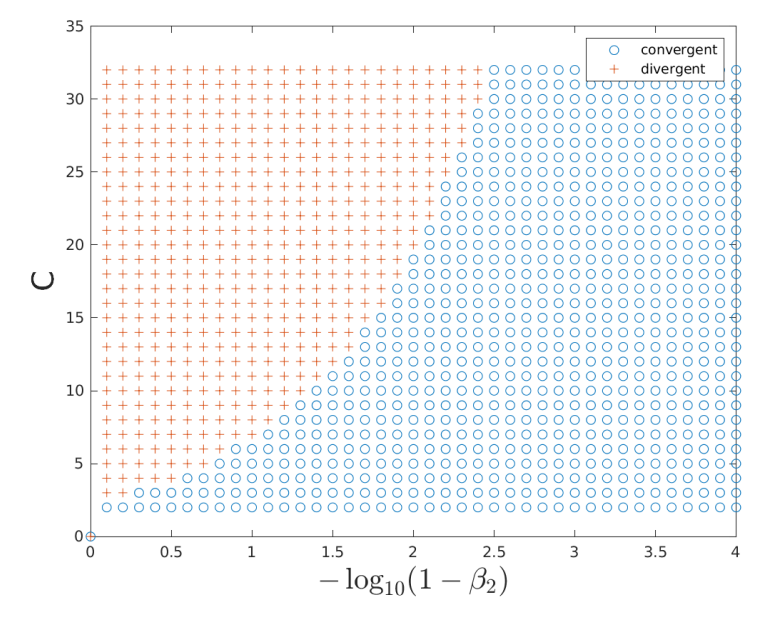
\includegraphics[scale = 0.4]{rmsp.png}
\caption{Phase diagram of the outcome of RMSProp on the counter example with the definition
			\(f_t(x) =
	\begin{cases}
		Cx & \ \ \text{for $t$ mod $C = 1$}\\
		-x & \ \ \text{Otherwise}\\
	\end{cases}
	\). 
	Different marks represent
	different outcome: we label a data point as convergence if the distance between $x$ and $-1$ is smaller than 0.01
	on average after 750000 iterations and as divergence otherwise. For each choice of $\beta$, there exists a counter
	example, but for each counter example in which Adam diverges, there exists a larger $\beta$ that can make Adam
	converge. Step size is set as $\alpha_t = \frac{1}{\sqrt{t}}$.}
\end{figure}
\begin{corollary}
	\label{coro51appendix}
	Let all assumptions in Theorem 5.2 hold. In addition, assume $D_0 = 0$ in (\hyperref[eq51]{1}), then for stochastic RMSProp we have,
	\[
	\min_{t \in (1, T]} \|\tilde{g}_t\|_1 \leq \mathcal{O}\Big(\frac{\log T}{\sqrt{T}}\Big), \ \ \ \forall \ T \geq 4
	\]
\end{corollary}
\begin{figure}[h]
	\label{fig2}
	\centering
	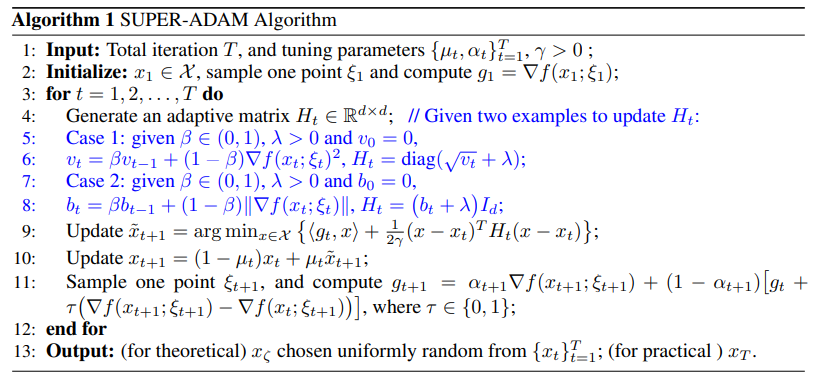
\includegraphics[scale = 0.5]{super-adam-algo.png}
	\caption{SUPER-ADAM Algorithm}
\end{figure}
\begin{corollary}
	\label{coro61appendix}
	In SUPER-ADAM algorithm, when $X=\mathbb{R}^d$ and given $\mu_t = \frac{k}{(m+t)}^{1/3}$ and $\alpha_{t+1} = c\mu^2_t$ for all $t\geq 0, \gamma = \frac{\rho m^{1/3}}{vkL}(v\geq 4), \frac{1}{k^3} + \frac{10L^2 \gamma^2}{\rho^2}\leq c \leq \frac{m^{2/3}}{k^2},
	m\geq\max(\frac{3}{2}, k^3, \frac{8^{3/2}}{(3k)^{3/2}})$ and $k > 0$, we have
	\begin{equation}
		\frac{1}{T}\sum^T_{t=1}\mathbb{E}||\nabla f(x_t)||\leq
		\frac{\sqrt{\frac{1}{T}\sum^T_{t=1}\mathbb{E}||H_t||^2}}{\rho}
		\left(\frac{2\sqrt{2G'}}{T^{1/2}} + \frac{2\sqrt{2G'}}{m^{1/6}T^{1/3}}\right),
	\end{equation}
	where $G'=vL(f(x_1) - f^*) + \frac{v^2 \sigma^2}{8} + \frac{v^2 k^4 c^2 \sigma^2}{4m^{1/3}}\ln(m+T)$.
\end{corollary}
\textbf{Remark A.2} \label{rmka2} WLOG, let $\rho = O(1), k = O(1), m = O(1), \gamma = O(1)$, we have $c=O(1)$ and $G = O(c^2 \sigma^2 \ln(m+T)) = \tilde{O}(1)$. Thus, our algorithm has a convergence rate of $\tilde{O}\left(\frac{1}{T^{1/3}}\right)$.
Let $\frac{1}{T^{1/3}}\leq \epsilon$, we have $T\geq \epsilon^{-3}$. Since SUPER-ADAM only requires computing two stochastic gradients at each iteration (e.g., only need tocompute stochastic gradients $\nabla f(x_{t+1}; s_{j_{t+1}})$
and $\nabla f(x_t; s_{j_{t+1}})$ to estimate $g_{t+1}$), and needs $T$ iterations. Thus, SUPER-ADAM ($\tau = 1$) has a gradient complexity of $2T = \tilde{O}(\epsilon^{-3})$ for finding an $\epsilon$-stationary point.
\begin{corollary}
	\label{coro62appendix}
	In SUPER-ADAM algorithm, when $X=\mathbb{R}^d$ and given $\mu_t = \frac{k}{(m+t)^{1/2}}, \alpha_{t+1} = c\mu_t$ for all $t\geq 0, k > 0, \gamma = \frac{\rho m^{1/2}}{vLk}(v\geq 8), \frac{8L\gamma}{\rho}\leq c \leq \frac{m^{1/2}}{k}$, and $m\geq k^2$, we haev
	\begin{equation}
		\frac{1}{T}\sum^T_{t=1}\mathbb{E}||\nabla f(x_t)||\leq
		\frac{\sqrt{\frac{1}{T}\sum^T_{t=1}\mathbb{E}||H_t||^2}}{\rho}
		\left(\frac{2\sqrt{2M'}}{T^{1/2}} + \frac{2\sqrt{2M'}}{m^{1/4}T^{1/4}}\right),
	\end{equation}
	where $M'=vL(f(x_1) - f^*) + 2v\sigma^2 + 2vm\sigma^2 \ln(m+T)$.
\end{corollary}
\textbf{Remark A.3} \label{rmka3} WLOG, let $\rho = O(1), k = O(1), m = O(1), \gamma = O(1)$, we have $M = O(\sigma^2 \ln(m+T)) = \tilde{O}(1)$. Thus, our algorithm has convergence rate of $\tilde{O}\left(\frac{1}{T^{1/4}}\right)$.
Considering $\frac{1}{T^{1/4}}\leq\epsilon$, we have $T\geq\epsilon^{-4}$. Since our algorithm requires computing a stochastic gradient at each iteration and needs $T$ iterations, SUPER-ADAM ($\tau = 0$) has a gradient complexity of $T = \tilde{O}(\epsilon^{-4})$ for finding an
$\epsilon$-stationary point.
\begin{figure}[h]
	\label{fig3}
	\centering
	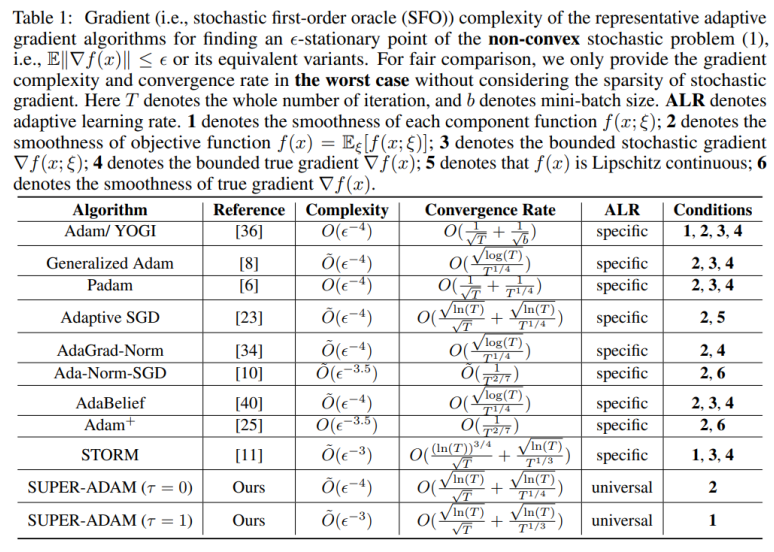
\includegraphics[scale = 0.5]{super-adam-comparison-table.png}
	\caption{Gradient Complexities of SUPER-ADAM and Other Algorithms}
\end{figure}
\end{document}
